
\chapter{Results and Discussion}
\begin{refsection}

This chapter presents the detailed development process, results, and evaluation of the Retrieval-Augmented Generation (RAG) chatbot developed for efficient literature search and thesis retrieval at the Camarines Sur Polytechnic Colleges (CSPC) Library. The chapter follows the system’s conceptual framework, covering data collection, preprocessing, indexing, query handling, response generation, output, and performance evaluation. All activities described were completed during the study period.

\section{Implementation of the Proposed Original Model}
This section outlines the development of the RAG chatbot system, which was guided by an integrated architectural framework comprising seven key stages. The figure below illustrates the complete system pipeline.

\begin{figure}[h]
    \centering
    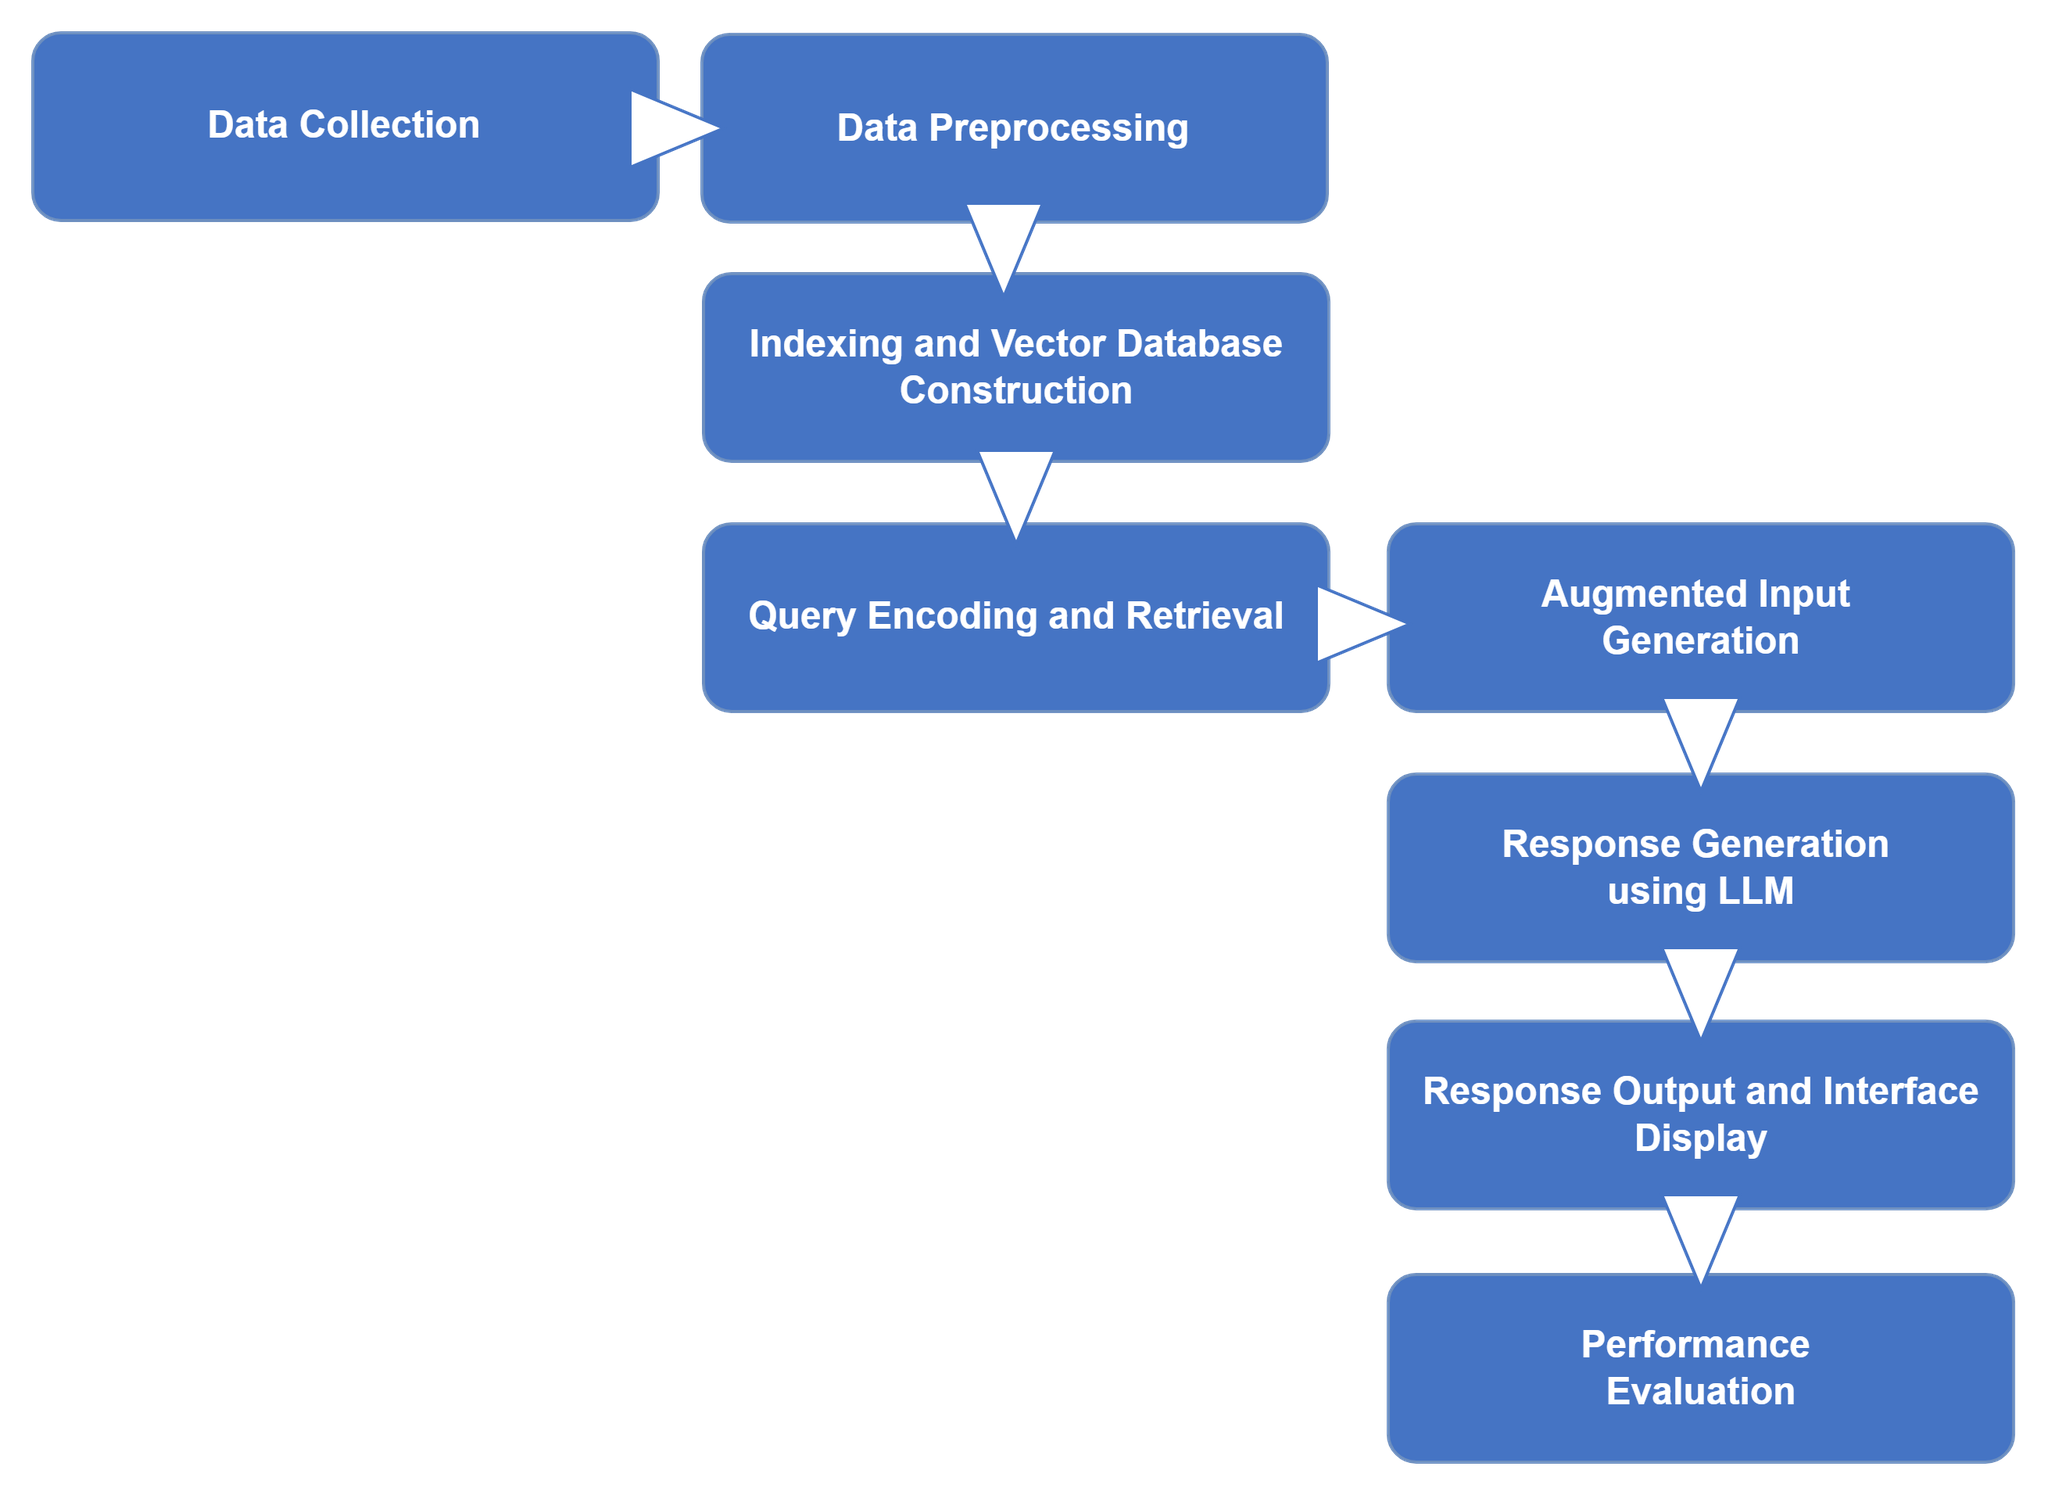
\includegraphics[width=0.7\textwidth]{figures/framework.png}
    \caption{Implementation of the Proposed Original Model}
\end{figure}

\section{Data Collection}
In this section, the researchers began with their proposal and coordination with CSPC Library and its staff, where the prototype was demonstrated to show how a RAG-powered chatbot could improve thesis discovery beyond exact-keyword search by enabling topic-oriented, semantically grounded retrieval within the library’s own repository. In the demonstration, the project’s institutional value was emphasized in accelerating literature searches, increasing access to relevant local theses, and supporting academic guidance, following the researchers' formal request to obtain one hundred undergraduate thesis PDFs from various College departments of CSPC to use as the main corpus of the RAG chatbot application.

\begin{figure}[h]
    \centering
    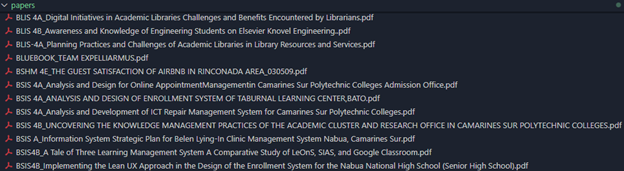
\includegraphics[width=0.7\textwidth]{figures/tsis_docs.png}
    \caption{CSPC Undergraduate Thesis Documents}
\end{figure}

Upon agreement on project scope, data handling practices, and local/on-premise deployment, library personnel granted the researchers to gain access to the digital copies of undergraduate thesis papers. The dataset was acknowledged and queued for the development phase following the proposed model pipelines’ process.

\subsection{Data Preprocessing}
This section commenced the systematic ingestion of the acquired thesis PDFs into the processing pipeline. Utilizing a custom script, the system recursively scanned the designated data folder housing more than 100 undergraduate thesis documents, ensuring all relevant files were accessed regardless of folder organization. Each PDF was processed page-by-page using the PyPDFLoader, extracting raw textual content alongside essential metadata such as source file paths and page numbers. This granular extraction maintained the academic formatting and pagination critical for preserving context, citations, and facilitating precise retrieval during later stages.

\begin{figure}[h]
    \centering
    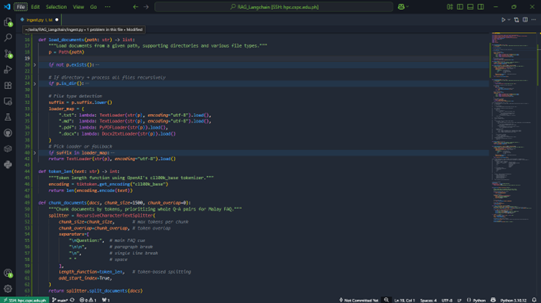
\includegraphics[width=0.7\textwidth]{figures/dtprprcss.png}
    \caption{Data Preprocessing inside the code editor}
\end{figure}

Extracted texts were segmented with a token-aware strategy (RecursiveCharacterTextSplitter), producing semantically coherent chunks sized to the LLM context window and guided by structural delimiters such as paragraph breaks and headings. Each chunk retained source, page, and positional offsets to support traceability and user navigation. The preprocessing yielded clean, contextually rich text segments ready for vectorization and indexing in the subsequent pipeline stage.    

\subsection{Indexing and Vector Database Construction}
The indexing phase transformed the preprocessed text chunks into a searchable knowledge base optimized for semantic retrieval within the RAG pipeline. This critical stage bridged the gap between raw textual content and the intelligent query-response capabilities that would define the chatbot's effectiveness in academic literature discovery.

\begin{figure}[h]
    \centering
    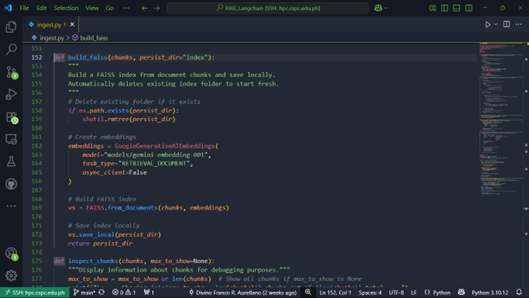
\includegraphics[width=0.7\textwidth]{figures/indfaiss.png}
    \caption{Indexing and Vector Database Construction}
\end{figure}

Each text chunk underwent embedding generation through the GoogleGenerativeAIEmbeddings model, which converted the semantic meaning of academic content into dense numerical vectors. This embedding process captured nuanced relationships between concepts, methodologies, and findings across the diverse corpus of CSPC thesis documents. The resulting vectors preserved both explicit textual information and implicit contextual relationships, enabling the system to understand queries about similar research topics, methodological approaches, or theoretical frameworks even when exact keywords differed. Following embedding generation, the vector representations were systematically indexed and stored within FAISS, a specialized library engineered for high-performance similarity search operations on dense vectors. The database construction process organized vectors using efficient indexing algorithms that would later enable rapid retrieval of contextually relevant thesis segments. Metadata preservation ensured that each vector maintained its connection to source documents, page numbers, and positional information, creating a comprehensive mapping between semantic concepts and their original academic contexts. This FAISS-based indexing architecture formed the retrieval foundation that would allow users to discover relevant thesis content through natural language queries, moving beyond traditional keyword matching to genuine semantic understanding of academic literature.


\subsection{Query Encoding and Retrieval}
The query processing stage represented the critical juncture where user intent transformed into actionable semantic search within the RAG chatbot system. This phase determined whether students and researchers would successfully locate relevant thesis content or encounter the frustrating "no results found" experience that plagued traditional keyword-based library systems.

\begin{figure}[h]
    \centering
    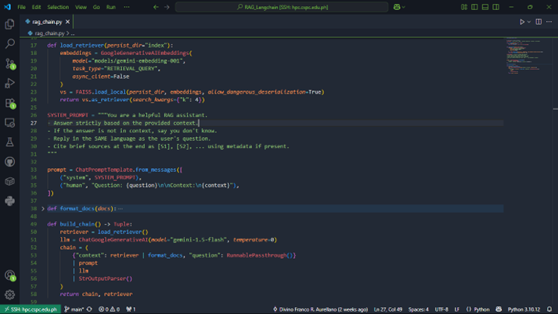
\includegraphics[width=0.7\textwidth]{figures/qandcntxtret.png}
    \caption{Question and Context Retrieval}
\end{figure}

When users submitted natural language queries such as "What research has been done on machine learning applications in healthcare?" or "Show me theses about sustainable energy solutions," the system initiated a sophisticated encoding process that mirrored the document preprocessing methodology. The user's question underwent vectorization using the identical GoogleGenerativeAIEmbeddings model employed during the indexing phase, ensuring semantic consistency between query representation and document storage. This encoding process transformed colloquial academic inquiries into dense numerical vectors that captured not just keywords but the conceptual intent and contextual nuances embedded within the user's research interests.

The retrieval mechanism leveraged the FAISS index infrastructure to execute high-speed similarity comparisons between the encoded query vector and the comprehensive collection of stored thesis document vectors. Using cosine similarity algorithms, the system calculated semantic distances to identify document chunks that most closely aligned with the user's informational needs. The top-K most relevant chunks—typically configured to retrieve four highly pertinent segments—were systematically selected and prepared for downstream processing. This retrieval approach transcended simple keyword matching, enabling the discovery of academically relevant content even when users employed different terminology, conceptual frameworks, or research perspectives than those found in the original thesis documents. The retrieved chunks formed the contextual foundation that would guide the language model's response generation, ensuring that chatbot answers remained grounded in actual CSPC thesis content rather than general knowledge or potential hallucinations.


\section{Augmented Input Generation}
The augmented input generation phase served as the crucial bridge between retrieved thesis content and intelligent response formulation, where raw document chunks evolved into contextually enriched prompts capable of guiding accurate academic discourse. Following successful retrieval of the top-K relevant thesis segments, the system executed a sophisticated concatenation process that preserved both content integrity and source attribution. Each retrieved document chunk underwent formatting that maintained its semantic value while incorporating lightweight citation markers such as to ensure academic provenance remained traceable throughout the response generation process. This formatting approach created a unified context string that seamlessly wove together diverse thesis excerpts, methodological discussions, and research findings into a coherent knowledge foundation.

\begin{figure}[h]
    \centering
    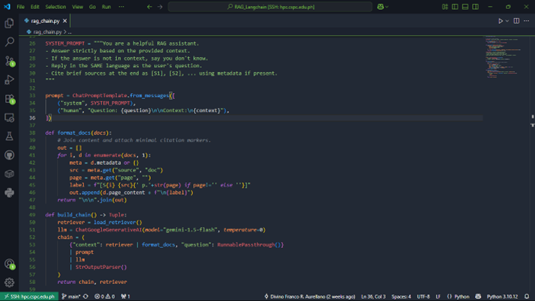
\includegraphics[width=0.7\textwidth]{figures/augInGen.png}
    \caption{Augmented Input Generation}
\end{figure}

The augmented prompt construction represented the culmination of the retrieval pipeline, where user queries and retrieved contexts merged into comprehensive input structures designed to optimize LLM performance within academic constraints. The system employed structured prompt templates to orchestrate a dual-component input framework consisting of system-level instructions that established academic rigor expectations and human-readable messages that combined the original user question with the formatted context string. This architectural approach ensured that the language model would receive explicit guidance to ground responses exclusively in provided thesis content while maintaining proper source citation practices. The pipeline incorporated practical safeguards, including token limit monitoring to prevent context overflow, intelligent truncation strategies for extensive retrievals, and explicit "no context available" indicators when insufficient relevant material existed, thereby maintaining input quality and preventing downstream processing issues.

\subsection{Response Generation}

The response generation stage represented the culmination of the RAG pipeline, where gemini-1.5-flash transformed augmented academic context into coherent, factually grounded answers that addressed user research inquiries. At this critical juncture, the language model processed the carefully constructed prompt containing both the original user question and the retrieved thesis content, leveraging its advanced reasoning capabilities to synthesize information from multiple academic sources into comprehensive responses. The system configured gemini-2.5-flash with temperature=0 to ensure deterministic output generation, eliminating randomness in responses and providing consistent answers when identical queries were posed. This deterministic approach proved essential for academic applications where reliability and reproducibility were paramount concerns for CSPC Library users seeking dependable research assistance.

\begin{figure}[h]
    \centering
    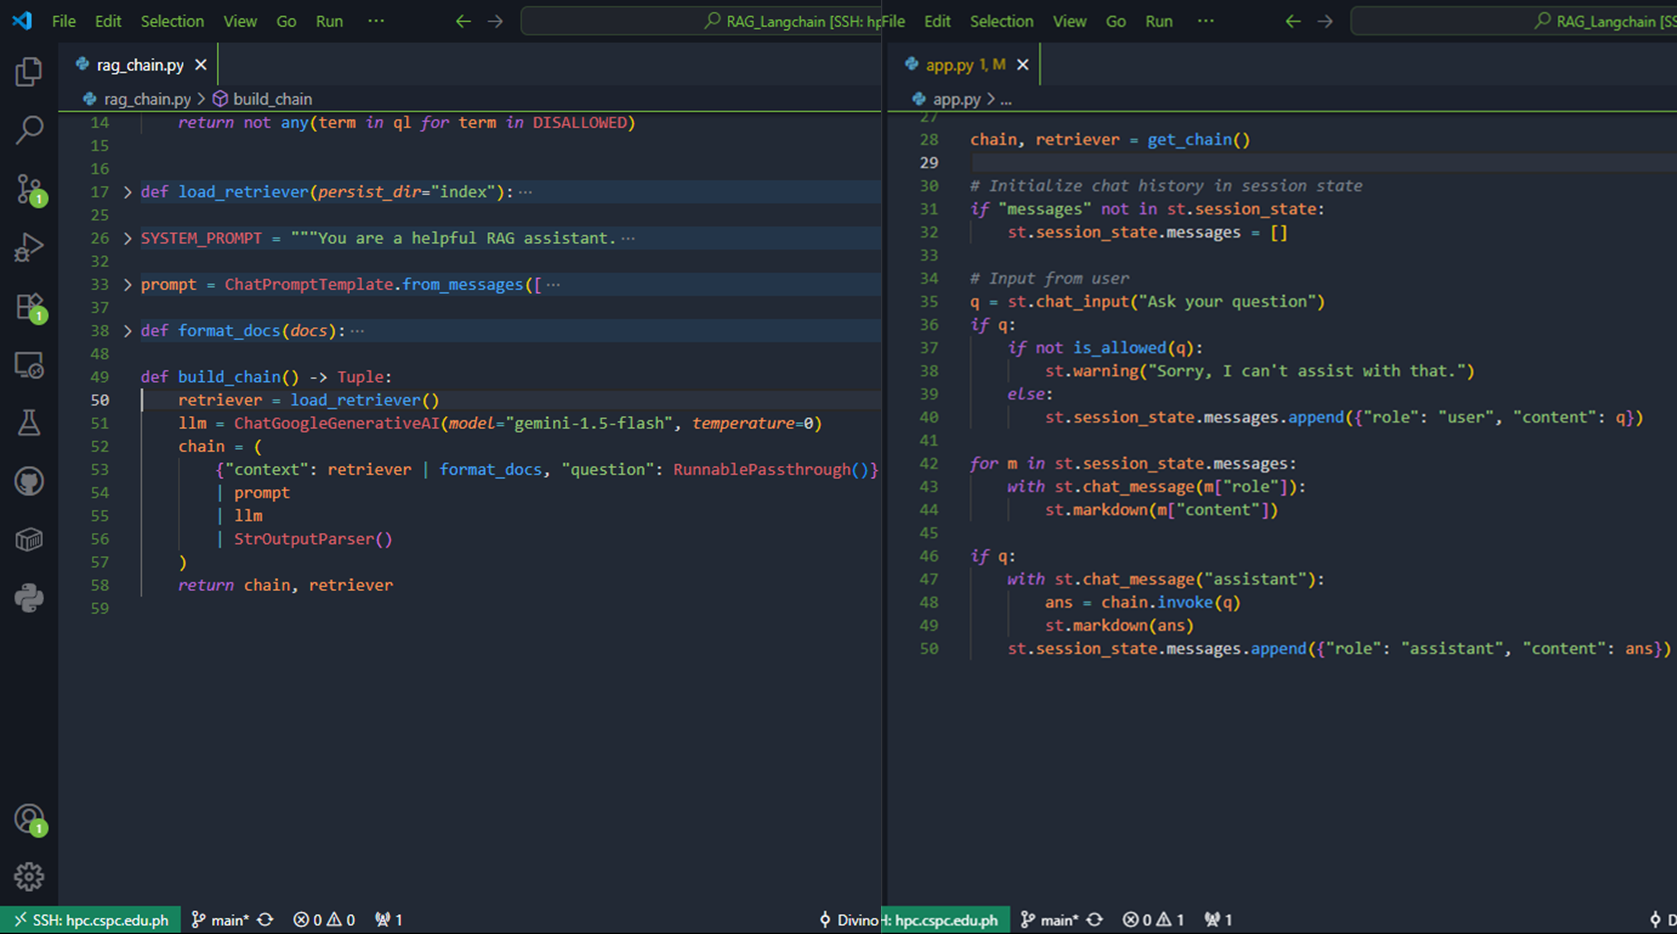
\includegraphics[width=0.7\textwidth]{figures/resgen.png}
    \caption{Response Generation}
\end{figure}   

The generation process operated through token-by-token prediction, where gemini-2.5-flash conditioned each response element on both the explicit system instructions and the augmented context, ensuring that generated content remained faithful to the retrieved thesis material rather than relying solely on pre-training knowledge. The model's reinforcement learning enhancements enabled sophisticated reasoning patterns that could identify relationships between different thesis segments, synthesize findings across multiple documents, and present information in academically appropriate formats. Following generation completion, the raw model output underwent parsing to yield clean text responses suitable for display within the chatbot interface. Despite the RAG framework's significant reduction in hallucination risks, the system maintained awareness that occasional inaccuracies could still occur when context was ambiguous or insufficient, necessitating user validation of critical research findings and encouraging cross-referencing with original source materials for comprehensive academic work.

\section{Response Output and Interface Display}

The final stage of user interaction materialized through a carefully designed Streamlit-based interface that transformed complex RAG processing into an intuitive conversational experience for CSPC Library users. When students and researchers submitted queries through the chat input interface, the system initiated a multi-layered safety and processing protocol that ensured both user protection and response quality. The application first executed content filtering mechanisms to verify query appropriateness before recording user messages in the session state, maintaining conversation continuity while preventing potentially harmful or inappropriate requests from reaching the underlying language model. This safety-first approach reflected the academic context where responsible AI deployment was essential for maintaining institutional standards and user trust.

\begin{figure}[h]
    \centering
    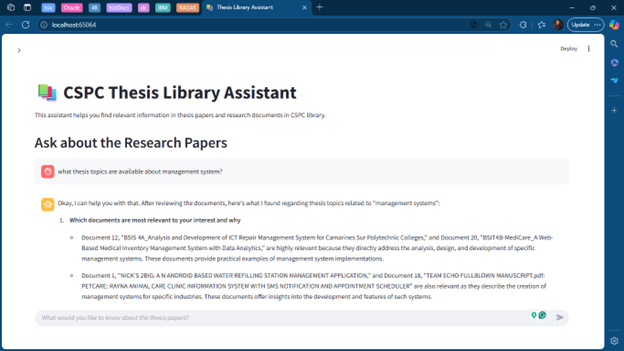
\includegraphics[width=0.7\textwidth]{figures/streamlit.png}
    \caption{Streamlit Interface Display}
\end{figure}

Following successful query validation, the cached RAG chain executed the complete retrieval and generation workflow through a single invoke call that orchestrated document retrieval, context formatting, and LLM response generation in a seamless pipeline. The interface architecture preserved conversation history by maintaining all user and assistant interactions within the session state, enabling users to reference previous exchanges and build upon earlier research discussions throughout extended library sessions. Generated responses appeared as rendered Markdown content that supported academic formatting including citations, lists, and structured text presentation, while the lightweight citation markers embedded within retrieved context enabled users to trace answers back to specific thesis documents and page references. When queries violated safety parameters, the system displayed clear Streamlit warnings instead of processing requests, maintaining transparent communication about system limitations. The synchronous processing approach with deterministic temperature settings ensured consistent response quality and eliminated unpredictable variations that could undermine user confidence in the academic research tool, while the persistent conversation interface encouraged iterative inquiry and deeper exploration of CSPC's thesis repository through natural dialogue.

\section{Model Evaluation}
In this section, the RAG-based chatbot system for the CSPC Library was evaluated utilizing four critical metrics: Answer Relevancy, Context Precision, Context Recall, and Faithfulness. These metrics provide a multidimensional perspective on the performance of the literature retrieval system, ensuring robust analysis in both information quality and reliability. The evaluation framework and explanations are patterned after established academic standards as demonstrated in the reference thesis.

\section{Result}
This section presents the findings through tables, figures, and subsequent discussion. Prior to evaluation, a systematic data processing pipeline was applied: 200+ undergraduate thesis PDFs from the CSPC Library were processed into segmented meaningful text chunks, and embedded using Hugging Face's Embeddings. These chunks were indexed in FAISS for efficient semantic retrieval, enabling the RAG chatbot to generate contextually relevant and factually grounded responses for user queries. This process ensured that the evaluation was conducted on high-quality, well-structured academic data.

\begin{table}[H]
    \centering
    \caption{RAG System Evaluation Metrics}
    \begin{tabular}{|l|c|}
        \hline
        \textbf{Metric} & \textbf{Average Score} \\
        \hline
        Answer Relevancy   & 0.737 \\
        Context Precision  & 0.818 \\
        Context Recall     & 0.721 \\
        Faithfulness       & 0.585 \\
        \hline
    \end{tabular}
\end{table}

\noindent The table above provides a concise summary of the RAG system’s evaluation metrics, offering a clear view of its performance in literature search and thesis retrieval tasks. Each metric captures a distinct aspect of the system’s effectiveness:

\begin{enumerate}
\item \textbf{Answer Relevancy (0.737):} This metric reflects how well the system’s responses address user queries. A score of 0.737 indicates that the chatbot generally provides answers that are relevant and useful, supporting users in finding the information they seek.
\item \textbf{Context Precision (0.818):} Context precision measures the proportion of retrieved text chunks that are actually relevant to the query. With a high score of 0.818, the system demonstrates strong ability to filter out irrelevant information, ensuring that users receive focused and meaningful content.
\item \textbf{Context Recall (0.721):} This metric assesses the system’s ability to retrieve all relevant information needed to answer a query. A score of 0.721 suggests that the chatbot successfully gathers most of the necessary supporting content, though there is still room for improvement in capturing every relevant detail.
\item \textbf{Faithfulness (0.585):} Reflects how accurately the chatbot's generated responses were supported by the source documents. While lower than other metrics, this value highlights a key area for improvement, emphasizing the challenge of maintaining strict factual consistency in generative retrieval systems.
\end{enumerate}

\noindent These metrics offer a comprehensive view of the system’s effectiveness. High answer relevancy and context precision demonstrate the chatbot’s practicality and efficiency in delivering relevant results, while context recall and faithfulness underscore the system’s coverage and reliability. Faithfulness, in particular, remains an ongoing focus for enhancement, aligning with current research advances in AI literature retrieval. These metrics collectively form the foundation for interpreting, tuning, and extending the RAG chatbot’s capabilities within the CSPC Library environment.

\begin{figure}[h]
    \centering
    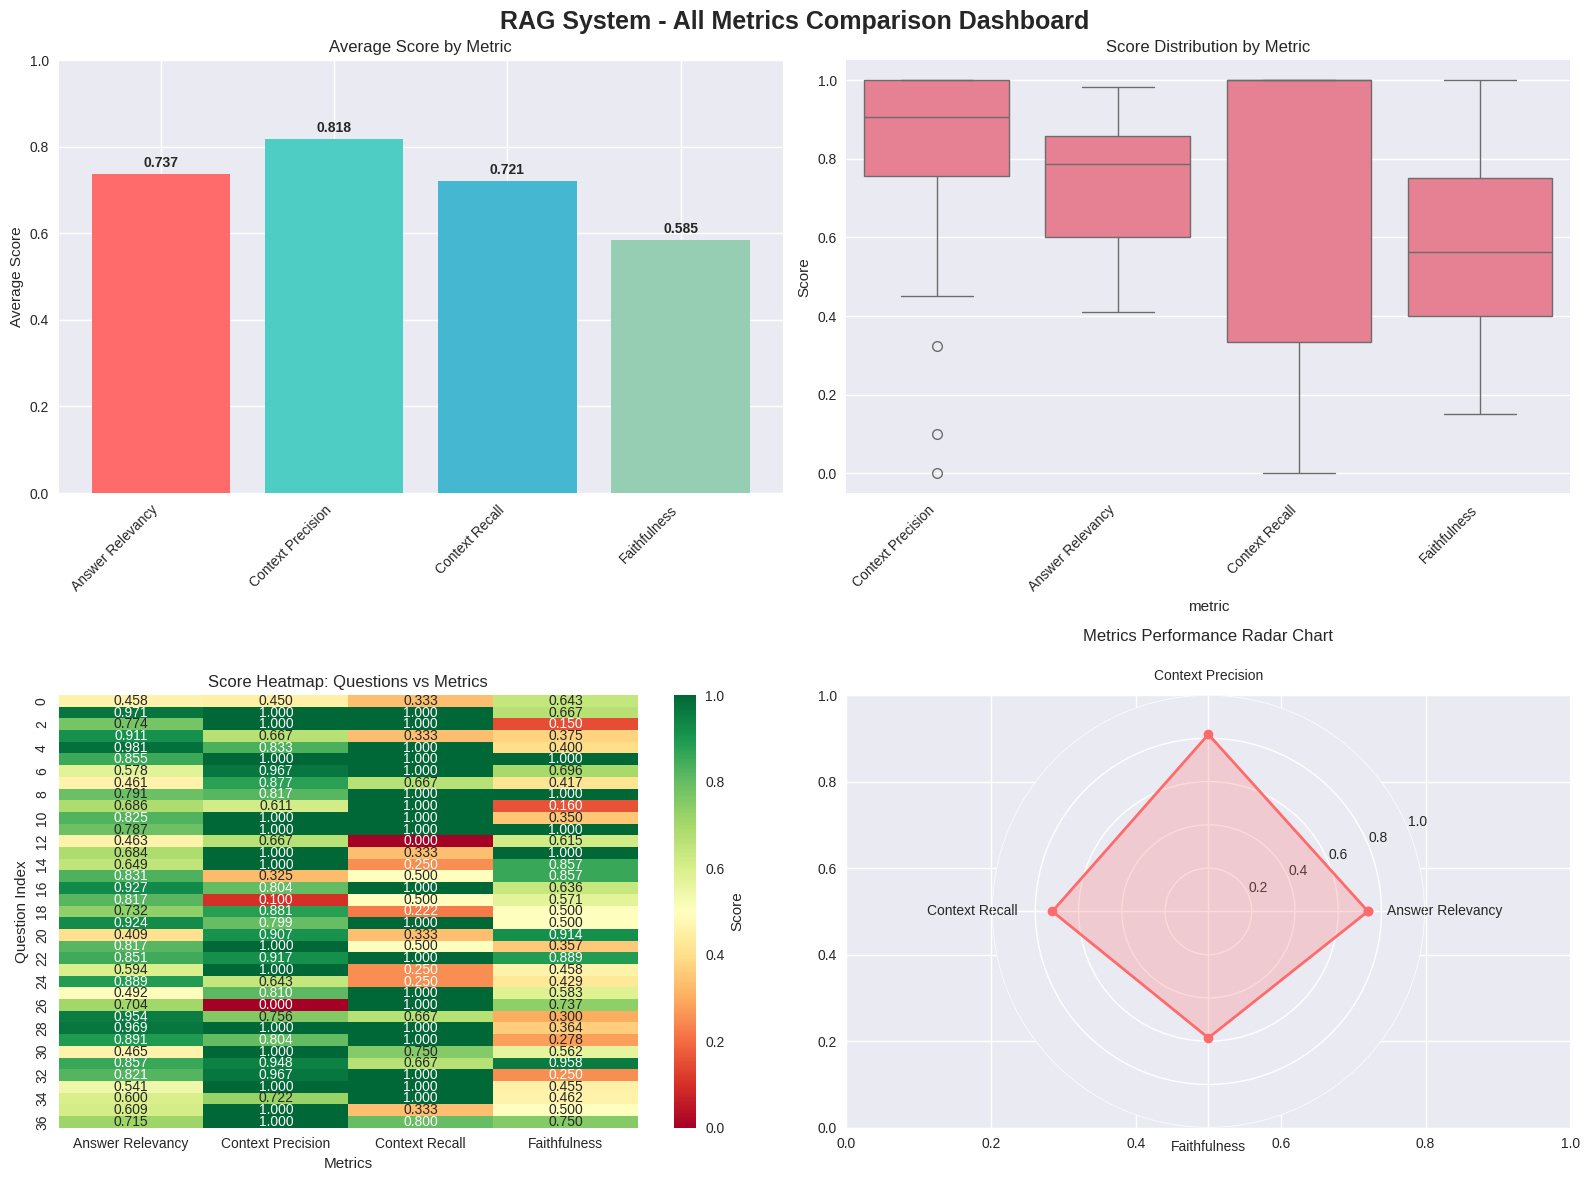
\includegraphics[width=0.7\textwidth]{figures/overall_out.png}
    \caption{RAG System - Metrics Dashboard}
\end{figure}

\section*{RAG System - Metrics Dashboard}
The dashboard presented herein serves as an integrated visualization tool for evaluating the RAG system’s performance across four core metrics: Answer Relevancy, Context Precision, Context Recall, and Faithfulness. Each chart within the dashboard offers unique insights into different aspects of system behavior in the context of literature search and thesis retrieval.
\noindent The bar chart illustrates the average score attained for each metric. Notably, Context Precision achieves the highest average (0.818), followed by Answer Relevancy (0.737), Context Recall (0.721), and Faithfulness (0.585). This ordering highlights the system’s exceptional ability to retrieve relevant information, moderate competence in delivering complete and relevant answers, and a comparative need for improvement in grounding generated responses strictly within the source material.
\noindent The box plot details the score distribution across metrics, emphasizing both consistency and spread. Metrics such as Context Precision and Answer Relevancy display less variance and higher minimum scores, indicating stable system performance. In contrast, Context Recall and Faithfulness exhibit a broader range, evidencing occasional lapses in comprehensive retrieval and accurate grounding.
\noindent The heatmap provides a granular view by displaying metric scores for individual questions. Darker shades correspond to higher scores, meaning better performance for both retrieval and generation on those specific queries. The heatmap reveals that while the chatbot excels on many questions, there is still inconsistency—some queries show lower faithfulness or recall, suggesting targets for further system refinement.
\noindent The radar chart synthesizes the metric scores into a single shape, depicting the RAG system’s overall performance profile at a glance. The profile is robust in Context Precision and Answer Relevancy, slightly reduced in Context Recall, and tapers at Faithfulness. This visualization makes clear where the system currently excels and where enhancements should be prioritized.

These visualizations collectively deliver a comprehensive, multi-faceted overview of the RAG chatbot’s strengths and areas for further enhancement. The visualizations reveal the system’s strong retrieval precision and relevancy, adequate recall, and opportunities for improvement regarding faithfulness to source documents. These insights guide ongoing refinements to optimize the chatbot for reliable, accurate, and comprehensive academic information retrieval.

%=======================================================%
%%%%% Do not delete this part %%%%%%
\clearpage

\printbibliography[heading=subbibintoc, title={\centering Notes}]
\end{refsection}